\documentclass{article}
\usepackage[utf8]{inputenc}
\usepackage[english]{babel}
\usepackage[cache=false]{minted}
\usepackage{graphicx}
\graphicspath{ {./images/} }

\title{Errors and Debugging}
\author{Guillaume Macneil}

\begin{document}
\maketitle

\begin{abstract}
This is the sixth lesson on the 'Introduction to Python' course, created by myself and Ariel Harmoko. This course is loosely based around the 'MIT Introduction to Computer Science - Fall 2016' course. Our course is more focused towards the Python programming side of things.
\end{abstract}

\section{Errors}
I'm sure that while following this course doing some programming of your own, you have encountered one or two errors. They are an inevitability of programming and should be seen as a programmer's friend, not enemy. In essence, errors are the computer saying "Whoa there, slow down. I can't do that." - they are guidance as to how you should write your code safely. If, by some miracle, you have never seen an error while programming in Python, here's an example of one: \medskip
\begin{center}
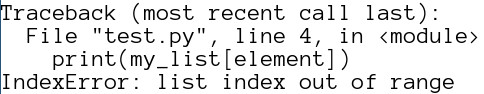
\includegraphics[scale=0.5]{example_error.jpg}
\end{center}
At first, this error may seem a little confusing, using made-up words like \textit{'Traceback'} and \textit{'IndexError'} or completely non-grammatical sentences like \textit{'most recent call last'}. They are however, quite useful and descriptive. For example, the above error was in response to the following code:
\begin{minted}{python}
my_list = ["Hello", "my", "name", "is", "Guillaume"]
for element in range(7):
    print(my_list[element])
\end{minted}
All of a sudden, the error message starts to make sense - I've iterated over a list of length 5, but I have tried to access all of the elements up to 7! There isn't even a 5\textsuperscript{th} element in the list to get to (because lists index from zero) let alone a 6\textsuperscript{th} or 7\textsuperscript{th}. So the sentence at the bottom of the error is actually saying \textit{'IndexError: You've tried to access an index that doesn't exist in \textbf{my\_list}'} - makes sense right? \medskip

It should come as no surprise though that \textit{IndexErrors} aren't the only kind of error Python has to offer, far from it. Here's a list of some of the basic ones that you will almost certainly come across during your Python programming career:

\begin{itemize}
    \item \textbf{SyntaxError} - Raised by the parser when improper language structure is used.
    \item \textbf{ImportError} - Raised when the imported module is not found.
    \item \textbf{IndexError} - Raised when the index of a sequence (list, tuple, etc.) is out of range.
    \item \textbf{KeyError} - Raised when a key is not found in a dictionary.
    \item \textbf{KeyboardInterupt} - Raised when the user presses the interrupt sequence (\textbf{Ctrl + C}).
    \item \textbf{MemoryError} - Raised when an operation runs out of memory.
    \item \textbf{NameError} - Raised when a variable cannot be found in the accessible scope.
    \item \textbf{IndentationError} - Raised when there is incorrect indentation
    \item \textbf{TypeError} - Raised when a function or operation is applied to an argument of incorrect type.
    \item \textbf{UnboundLocalError} - Raised when a local variable has been referenced, but has not been bound to a value.
    \item \textbf{ValueError} - Raised when a function is applied to an argument of correct type but incorrect value.
    \item \textbf{ZeroDivisionError} - Raised when the second operand of a division-related operation is zero.
    \item \textbf{RuntimeError} - Raised when the error does not fall under any other error name.
\end{itemize}
There are a few important things to note here: \textbf{1.} This list does not even begin to scratch the surface of the potential errors in Python, not only does it not list all of the core errors that the interpreter can return, it does not mention \textbf{any} of the custom errors raised by imported modules (a topic that will be explored further in the next lesson). \textbf{2.} You don't really need to learn these off by hert, if you come across an error that you don't know how to fix, just search it up on the internet - it is very, very rare to be the first person to come across a particular error. \textbf{3.} Some pedants would say \textit{'Well actually, most of the "Errors" that you listed there are actually "Exceptions". \textbf{Actually}.'} While these people are technically right, who cares.

\section{Debugging}
You may have heard of the term \textit{'bugs'} in the context of programming before. Bugs are mistakes in the way your program is written, which make it act in unwanted and unforeseen ways. Errors are a type of bug, in the sense that they make your program crash - which is almost never what you want. If we want our program to work, we need to mitigate the number of bugs there are in our programs. It is also important to note that the larger your program gets, the more bugs will appear and the harder it will be to remove them all. The key to making good programs is removing as many as you can and only leaving ones that have very little effect on the function of your code. With that said, there are three main stages to \textit{'squashing bugs'}:

\begin{itemize}
    \item \textbf{Before writing any code:} \\
    Make sure to write code in a way that is easily understandable for others and your future self. Though the variable name \textbf{iter\_A\_count\_1} may make perfect sense when you first write it, once you come across a bug that breaks something related to this awfully named variable, I can promise that it will be a headache trying to fix it. So do yourself (and others) a favour and name your variables, functions, classes and files in a way that \textbf{ describes what they do}.\medskip

    Secondly, split any reused code into functions and classes. Though it may seem like a purely academic exercise at first, it makes fixing bugs related to this code \underline{so much easier}.\medskip

    Finally, use comments to describe what your code does. Now this does not mean adding a comment in front of every line of code, describing its intricacies in boring detail. Just use the occasional comment to help remind the programmer what a block of code does.

    \item \textbf{While writing the code:} \\
    Frequently test your code while you are writing it. Many experienced programmers will tell you to use \textit{'unit tests'}, \textit{'regression tests'} and \textit{'integration tests'}. They'll tell you to use \textit{'black box testing'},\textit{'glass box testing'} and various other scary-sounding methods to squeeze every last bug out of your program. While these are undeniably useful in team environments and are certainly necessary in corporate environments where if your code breaks there are real, tangible consequences - I find that this kind of exhaustive approach removes all of the fun and flexibility from programming.\medskip

    The method that I use is to frequently test the code that I am writing with the any inbuilt \textit{debugger} and, more often than not, just \textit{print()} statements. This method ensures that everything returns the values that you want and generally works the way you want. It is often very useful to let the errors that you get guide the way you write your code, as the interpreter often knows what's best.

    \item \textbf{After writing the code:} \\
    If you have frequently tested the code while writing it, you will have very little to do here. At this point all you want to do is consider some test cases for the program you've written. What would be the general use-case for your code? Does it work well with this? What would be the extreme use-cases for your code? Can it handle that? What about the ways that your code shouldn't be used? Have you accounted for this? \medskip

    Those last two questions are often overlooked by beginners. Consider how your code will inevitably break, even if the use-case seems stupid. Leave messages and maybe even custom exceptions for the user so as to inform them that they shouldn't use the program like that.
\end{itemize}
Now, looking at a page of instructions like that is enough for anyone to say 'Alright, maybe programming isn't for me' and please note \textbf{I am not trying to tell you exactly what to do. These are merely pointers.} In the world of programming these types of instructions are called \textit{'best practices'}, and many new programmers (myself included) often find themselves following these so closely that they don't really learn anything for themselves - they just copy whatever they find on the internet without even questioning it. So my advice to you is to just try stuff out, see what works and do whatever you think works best for you. \textsubscript{\textbf{With that said though, my advice is good...}}

\section{Notes}
This section is only here to provide some context to my points, if you understood everything I said with perfect clarity, feel free to skip this section.
\subsection{Well-Named Code}

Here's an example of some (in my humble opinion) well-named code that is easily understandable for your future self and others.
\begin{minted}{python}
from random import randint

# A function that generates a random 8 digit, numerical code
def generate_code():
    code_string = ""
    for _num in range(8):
        code_string += str(randint(0, 9))
    return code_string
\end{minted}

As you can see, this code is relatively readable and easy to understand:
\begin{itemize}
    \item Only one function is imported (\textit{'randint'}) from the \textit{'random'} module, because only one is used.
    \item A comment is used to describe the what the function does.
    \item Each variable has an understandable name.
    \item Necessary, but unused variables are prefixed with an underscore (another 'best practice')
\end{itemize}

Though there are likely more efficient functions that could generate a random 8 digit code, I find it is generally at the expense of readability.
\subsection{Raising Custom Exceptions}

If want a function to return an error when it is used in such a way. You can do so with the \textit{raise} command:
\begin{minted}{python}
# Used like this: raise <exceptionName> (<arguments>)
raise TypeError("Only use objects of type: String")
raise RuntimeError("A very useful and descriptive message")
\end{minted}
\end{document}
